
Put your Experimental results
\section{Testing Frame Construction(FrameObj)}
%Rebecca
% not sure how much of this le will go over...so super brief here
An easy way of being able to integrate with the other teams seemed to be through the creation of a class, FrameObj, which would not only provide the other modules with a means of creating a frame but a list of properties that could be called for easy debugging. There are two ways that an instance of the class FrameObj could be constructed,  from the basic requirements of the frame (Frame type, Sender ID number , Receiver ID number, and Data) or from the bits of data that make up a frame.

4 sections of testing that done to frame object. 

section 1 tests the ways we can make an invalid frame








\section{End-to-End Local Machine Testing }
%Renato
The test of the implementation of the end to end communication.
Based on proposal of final design project \cite{cdproj}, there
are six case to be tested in the end to end communication
\begin{enumerate}
  \item Extra-cellular communications between UEs
  \begin{enumerate}
    \item US1 $\rightarrow$ BS1 $\rightarrow$ BS2 $\rightarrow$ US3
    \item US3 $\rightarrow$ BS2 $\rightarrow$ BS1 $\rightarrow$ US1
		\item US2 $\rightarrow$ BS1 $\rightarrow$ BS2 $\rightarrow$ US3
		\item US3 $\rightarrow$ BS2 $\rightarrow$ BS1 $\rightarrow$ US2
  \end{enumerate}
  \item Intra-cellular communications between UEs
	  \begin{enumerate}
    \item US1 $\rightarrow$ BS1 $\rightarrow$ US2
    \item US2 $\rightarrow$ BS1 $\rightarrow$ US1
	\end{enumerate}
\end{enumerate}

The figure \ref{fig:endendDiagram} show how the whole MATLAB code is organized to test all the cased described in this section.
The send and received part maps each path of information lie UE 1 to BS1 as a channel . It more logical representation that to a physical channel to the end
to end implementation in the final integration.
The routing used was just a siwtch case based on picture of proposed network in \cite{cdproj}.
The send and received is a recursive function that call it self based with parameters changed for the routing.
One examples is shown in listing \ref{sendReceiveExample} show how inside a channel based on direction how it will resend the message or exit the the function based on the destination.
\lstset{caption={Code examples how to verify the CRC and create the ACK message back to sender},label=sendReceiveExample}
\lstinputlisting{code/sendReceiveExample.M}

The listing \ref{crcVerification} is a examples how the receveive UE in the figure \ref{fig:endendDiagram} verify the CRC and create the new frame to send back.
It procedure is important because it need to be done in the integration with other team that need to use the frameObj.     

\lstset{caption={Code examples how to verify the CRC and create the ACK message back to sender},label=crcVerification}
\lstinputlisting{code/crcVerification.M}



\begin{figure}[ht]
    \centering
    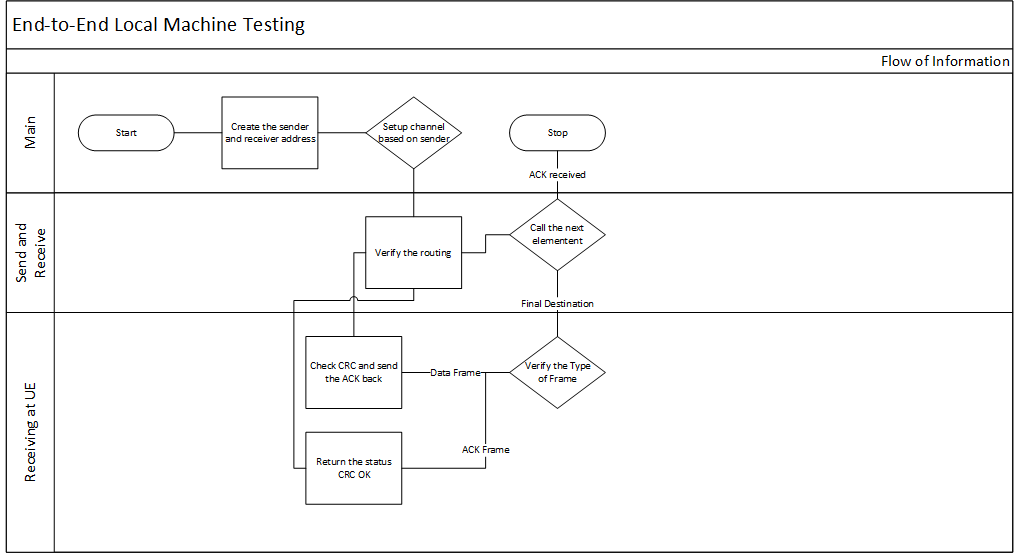
\includegraphics[width=0.8\textwidth]{flowEndtoEnd.PNG}
    \caption{Diagram of the flow of information to test the end to end in Matlab for the team 6 proposed protocol}
    \label{fig:endendDiagram}
\end{figure} 

\section{Transmitting and receiving over the air}
%Renato
The frame object need to be tested over the air to check if it behaves as expected in our simulation. 
It was tested using two different physical layer. 
\subsection{Using lab2 physical layer}
The first test was using a very straight forward approach. We just replaced the 'hello world' message in the Lab 2 
simulating model to add the frame object with a message 'Hi', so it can send a frame near the original size.
The code to create frame is shown in \ref{transLab02}. It is used as input of simulation in diagram of figure \ref{fig:trasmitter_lab02}.
\lstset{caption={Code to create the transmitter package to used in Lab 02 physical layer},label=transLab02}
\lstinputlisting{code/crcVerification.M}

\begin{figure}[ht]
    \centering
    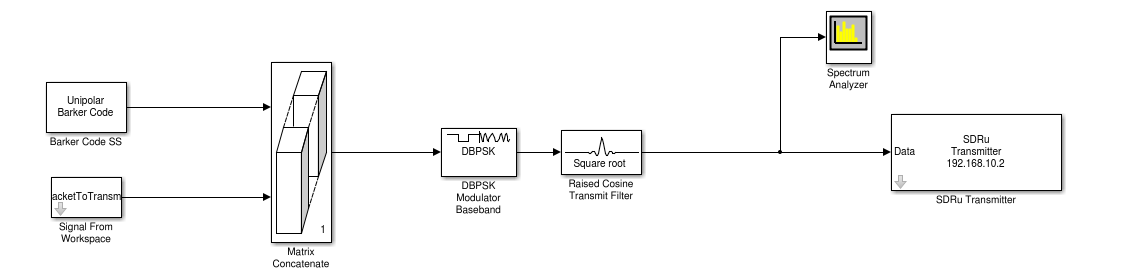
\includegraphics[width=0.8\textwidth]{trasmitter_lab02.PNG}
    \caption{Simulink diagram of the transmitter of the laboratory two physical layer modified to received a input frmaobje wit the message 'Hi' }
    \label{fig:trasmitter_lab02}
\end{figure}

The receiver changed also to verify the CRC and count the number of data frame,ack frame and invalid. The diagram of this receiver is
shown in figure \ref{fig:receiver_lab02}.

\begin{figure}[ht]
    \centering
    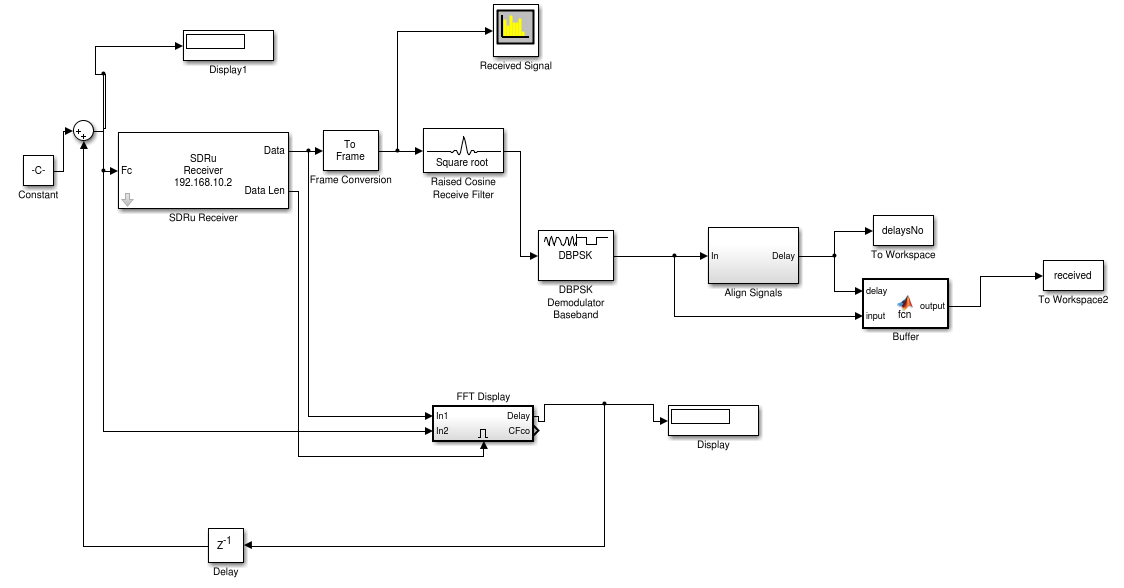
\includegraphics[width=0.8\textwidth]{receiver_lab02.PNG}
    \caption{Simulink diagram of the receiver of the laboratory two physical layer modified to received a a frame and verify the CRC and which frame type }
    \label{fig:receiver_lab02}
\end{figure}


The result have poor result. The table \ref{tab:2ACK} shows a FER around 97\% and had case of false detection of a ACK frame when the transmitted only send
the same data frame with 'Hi'.  


To avoid the false detection, we change the value of the Data Frame to 240 that is 1111 0000 in binary and the ACK frame to 255 that is 1111 1111.
The FER was still very high above 95\% but not ACK frame was detected as shown in Table \ref{tab:0ACK}. Increase the hamming distance of the numerical representation of Data frame and ACK frame 
fixed this false detection.
 




\begin{table}[ht]
	\centering
		\begin{tabular}{| c | c | }
		\hline                       
		Frame Type UE & Number Received\\
		\hline
			ACK & 2\\
			DATA & 102\\
			corrupt DATA & 2\\
			INVALID & 3466\\
			other & 0\\
		\hline
		\end{tabular}
	\caption{Table of frames received with poor transmission quality and a small hamming distance between frame types.The ACK was a false positive error because the frame type had a very close number}
	\label{tab:2ACK}
\end{table}

\begin{table}[ht]
	\centering
		\begin{tabular}{| c | c | }
		\hline                       
		Frame Type & Number Received\\
		\hline
			ACK & 0\\
			DATA & 165\\
			corrupt DATA & 4\\
			INVALID & 3559\\
			other & 0\\
		\hline
		\end{tabular}
	\caption{Table of frames received with poor transmission quality and a larger hamming distance between frame types}
	\label{tab:0ACK}
\end{table}

\subsection{Using Team 4 physical layer}
\label{team4_results}
To decrease the FER, we replaced the physical layer for one more robust taht have interleaving and bit repetition to improve the recovery of the information in the receiver side.
We used the Team 4 taht have all those features included and needed minor modification to transmit the frame Object instead of the original frame from Team 4.
The first modification is the size fo the block interleave to handle 8 bit word instead of 7 bits used from Team 4. We also changed the size of the padding because our message was smaller and we decide to keep the same output of 987 bits to added to 13 bits baker. The diagram of this transmitter is shown in figure \ref{fig:transmitter_team4}. Iti is very similar to the laboratory 02 , the main change is the size of buffer to fit the repeated and interleaved message.  
\begin{figure}[ht]
    \centering
    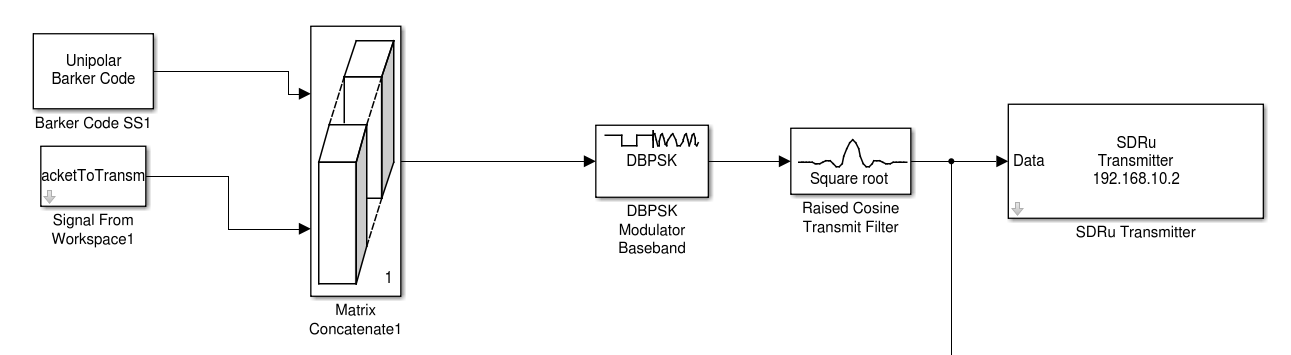
\includegraphics[width=0.8\textwidth]{transmitter_team4.PNG}
    \caption{Simulink diagram of the receiver of the laboratory two physical layer modified to received a a frame and verify the CRC and which frame type }
    \label{fig:transmitter_team4}
\end{figure}

The receiver diagram from figure \ref{fig:receiver_team4} is much more complex from laboratory 02 because Team 4 upgrade the delay detection and the frequency correction.
We made similar changes to revert the interleave and get the mean of the values of the repeated bits to recreate the data frame object.
We also make the bi directional transmission. We receive the data frame check CRC of the data part check. The performance of receiving data package is show in Table \ref{tab:team4data}. If at least one data packet is correct, we start one transmitter block like in figure \ref{fig:transmitter_team4} to send the ACK back to the other machine. The performance of receiving ack package is show in Table \ref{tab:team4ack} . If at Full code for this receiver is shown by the listing \ref{ReceiverTeam4Code} in the appendix. All this process was recoded and is available at \cite{videodemo}. 
 

\begin{figure}[ht]
    \centering
    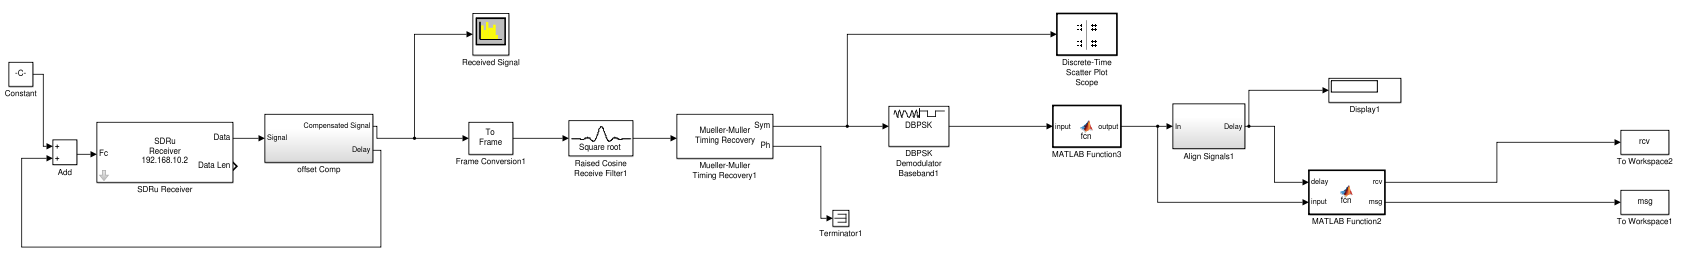
\includegraphics[width=0.8\textwidth]{receiver_team4.PNG}
    \caption{Simulink diagram of the receiver of the laboratory two physical layer modified to received a a frame and verify the CRC and which frame type }
    \label{fig:receiver_team4}
\end{figure}

\begin{table}[ht]
	\centering
		\begin{tabular}{| c | c | }
		\hline
			\multicolumn{2}{|c|}{Data Frame}\\
		\hline                       
			 Total frame received & 62\\
			 Correct frame received& 23\\
		\hline
			FER & 63\%\\
		\hline
		\end{tabular}
	\caption{Table of data frames received using the team 4 physical layer with repetition factor of 4 and block interleaving}
	\label{tab:team4data}
	\end{table}

\begin{table}[ht]
	\centering
		\begin{tabular}{| c | c | }
		\hline
			\multicolumn{2}{|c|}{ACK Frame}\\ 
		\hline                       
			 Total frame received & 66\\
			 Correct frame received& 37\\
		\hline
			FER & 44\%\\
		\hline
		\end{tabular}
	\caption{Table of ack frames received using the team 4 physical layer with repetition factor of 4 and block interleaving}
	\label{tab:team4ack}
	\end{table}